\documentclass[a4paper,12pt]{article}
\usepackage[utf8]{inputenc}
\usepackage{graphicx}
\usepackage{amsmath}
\usepackage{float}

\title{How has COVID impacted economic activity and what have been the extent of these impacts?}
\author{Terry Qi}

\begin{document}

\maketitle
\newpage
Word count:

Article: https://www.bbc.com/news/business-54186359, Covid pushes New Zealand into worst recession in years, 17/09/2020, published by the BBC, on 17/09/2020, accessed 27/10/2021

Topic Macroeconomics

Key Concept: Change


% planning
% gdp shrank 12.2% lockdown. first recession. impact on retail, accommodation, restaurations, transport, decline production travel bans.

% more research: inflation, unemployment, imports & exports, economic growth

\section*{Topic}
The article chosen discussed the impact of COVID-19 on the economy of New Zealand in 2020. It stated a measured 12.2\% decrease in the national nominal GDP, as well as classifying the status as ``the deepest recession in decades''. This discussion will focus on the change in the retail sectors of the economy through the application of economic theory, and will evaluate its broader impacts on the wider economy.

\section*{Theory}
As stated in the article, the pandemic had directly affected the retail industry in a perceived decrease in production quantity. This is very likely caused by various international travel bans and strict nationwide lockdowns.

% theory
\begin{figure}[H]
    \centering
    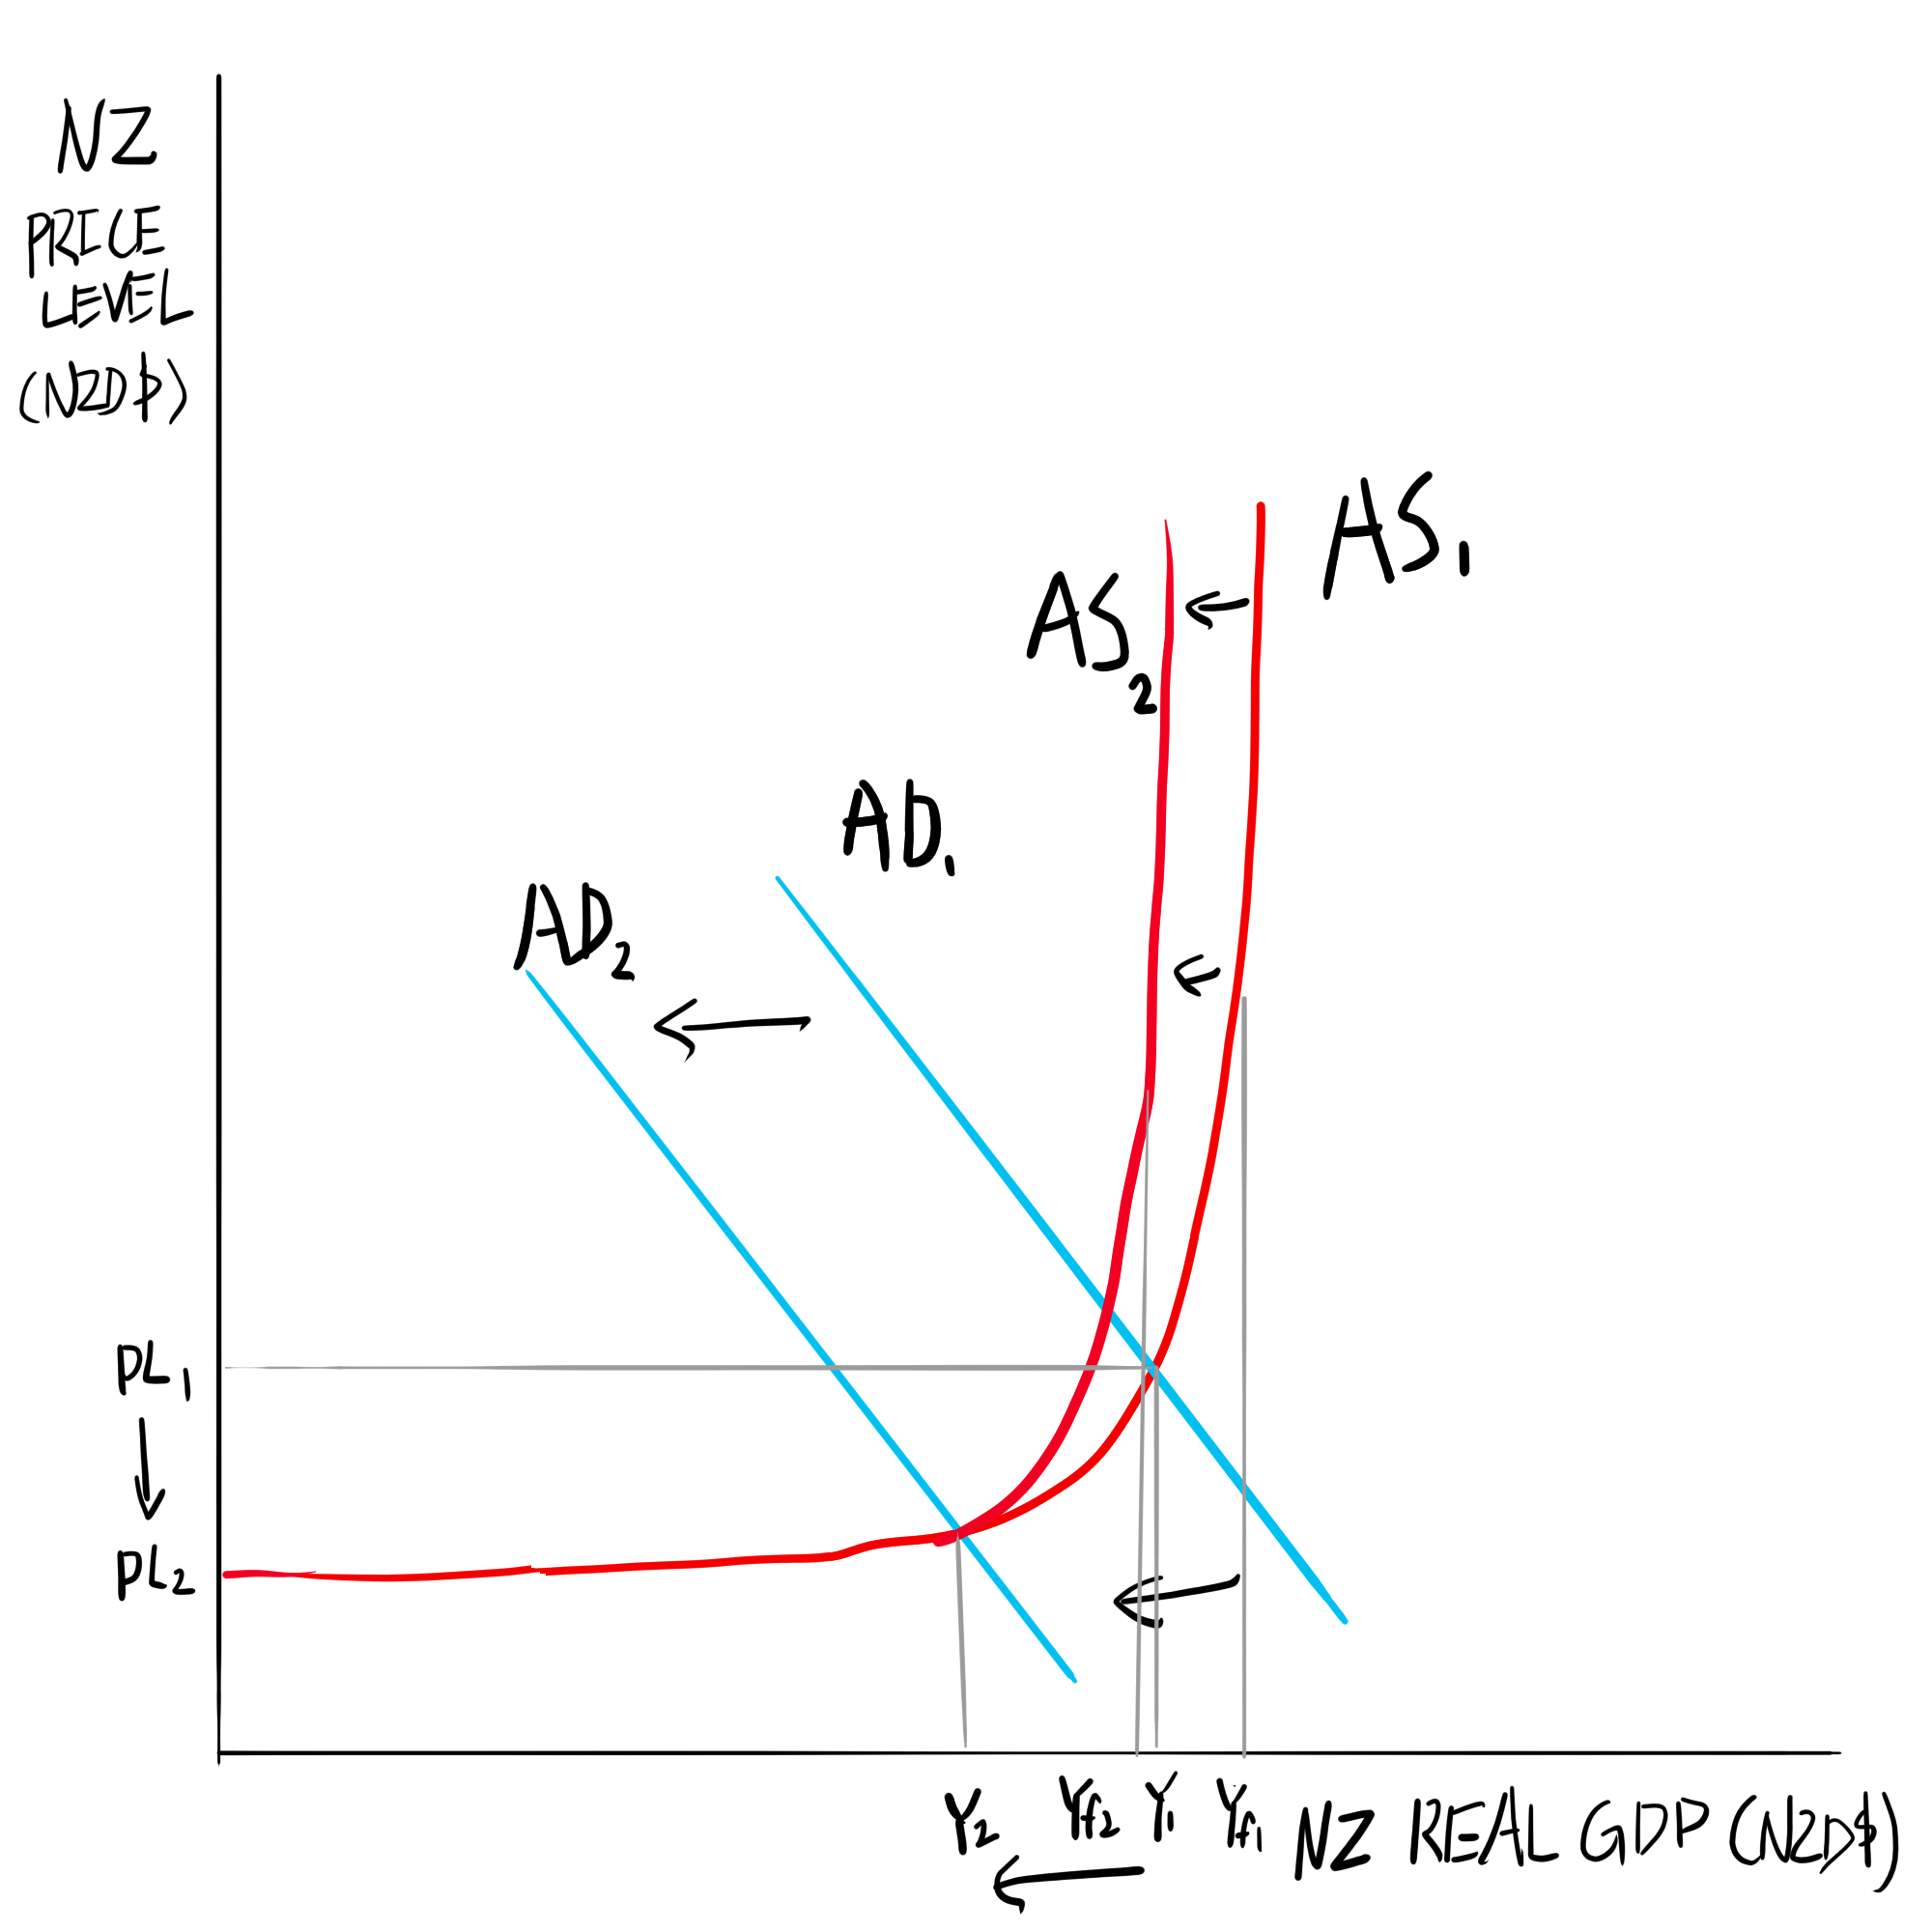
\includegraphics[scale=0.7]{assets/asad.png}
    \caption{The NZ economic diagram during COVID}
    \label{fig:asad}
\end{figure}

\section*{Evaluation}

% more stuff

\section*{Summary}

% end

\end{document}
